\documentclass[a4paper,10pt,titlepage]{article}
\usepackage[utf8]{inputenc}

% Handmade package to define patterns.
\usepackage{pattern}
% For the \todo{} command.
% \usepackage{todo}

% Nice fonts
\usepackage{palatino}
% Needed for Listings package with Eiffel.
\usepackage{xcolor}
% Source code listings.
\usepackage{listings}
% Appendix with extra title.
\usepackage [page] {appendix}
% To include PNG files.
\usepackage{graphicx}
% Nice looking captions.
\usepackage[font={footnotesize,sl}, labelfont=bf] {caption}
% Include PDF pages.
\usepackage{pdfpages}

% Clickable links. Has to be the last package:
\usepackage [hidelinks] {hyperref}


\lstset{language=OOSC2Eiffel,basicstyle=\ttfamily\small}
\definecolor{codebg}{rgb}{0.95,0.95,0.95}
\setlength{\headheight}{28pt}
\lstset{escapechar=\$}

\newcommand{\dir}{\emph}
\newcommand{\todoref}{\todo{ref}}

% Title Page
\title{Concurrency Patterns in SCOOP}
\author{Roman Schmocker \\ \\ Supervised by Alexey Kolesnichenko \\ and Prof. Dr. Bertrand Meyer}


\begin{document}
\pagenumbering{roman}

\includepdf {resources/titlepage}


\includepdf {resources/declaration_of_originality_signed}

\begin{abstract}
\thispagestyle{plain}
\setcounter{page}{3}
The wide distribution of multi-core processors increasingly forces programmers to deal with concurrency.
Parallel programming is not easy, but there are many well-known patterns at hand to help developers.

SCOOP, an extension to the Eiffel programming language, provides an alternative approach to concurrent programming compared to the threading mo\-del used in many other languages.
There is little experience in implementing and using concurrency patterns in SCOOP however.

We have investigated which patterns are used in practice and compiled an exhaustive list of pattern descriptions.
From this list we selected several popular concurrency patterns and implemented them as a reusable Eiffel library.
A small performance comparison shows that the new library is more robust and faster for large data sets than a raw SCOOP solution.
We also describe some of the challenges when programming in SCOOP for the first time and provide solutions.
\end{abstract}

\renewcommand{\abstractname}{Acknowledgements}
\begin{abstract}
\thispagestyle{plain}
\setcounter{page}{4}
I would like to thank Alexey Kolesnichenko very much for his great support and helpful advice throughout my thesis.
Many thanks go to Prof. Bertrand Meyer for his insightful comments and for giving me the opportunity to work on this project.
I would also like to thank Julian Tschannen, Mischael Schill, Scott West, Sebastian Nanz and others at the Chair of Software Engineering for their useful input.

\emph{Roman Schmocker}
\end{abstract}


\setcounter{page}{5}
\tableofcontents

% Blank page to make sure introduction starts on the right.
\newpage
\mbox{}

\newpage
\pagenumbering{arabic}

\section{Introduction}
\label{sec:introduction}


Due to the advent of multicore processors, concurrent programming has become an important part in software engineering.
Dealing with parallelism isn't easy however.
There are many pitfalls, such as race conditions and deadlocks.

In practice programmers have learned to avoid tricky concurrency problems with the use of some well-known patterns.
These patterns are often shipped as part of the standard library of the language, such that users rarely have to implement them.

The Eiffel programming language \cite{web:ecma-eiffel}\cite{book:touchofclass} has an extension called SCOOP \cite{Nienaltowski07}\cite{web:scoop},
which stands for Simple Concurrent Object-Oriented Programming.
SCOOP simplifies concurrent programming a lot and eliminates one source of errors completely, namely race conditions \cite{Nienaltowski07}.
However, there is little experience on how to implement popular concurrency patterns, like a worker pool, in SCOOP.

This thesis tries to fill this gap by providing a library of reusable concurrency patterns as well as methodical advice on programming in SCOOP.
The main contributions are:
\begin{itemize}
 \item A broad survey of known concurrency patterns.
 \item The identification of common SCOOP challenges and advice on how to solve them.
 \item A new library which provides implementations for some selected concurrency patterns.
 This selection was mainly based on input from the Software Engineering group at ETH Zürich and the study of Java \cite{web:java-concurrency} and C\# \cite{web:ms-tpl} concurrency libraries.
\end{itemize}

\subsection{Overview}

Section \ref{sec:pattern_overview} introduces a list of concurrency patterns which we found and categorized by studying literature and the standard libraries.
A brief introduction of the SCOOP model is given in Section \ref{sec:scoop-model}.
Section \ref{sec:scoop-challenges} describes some challenges when programming in SCOOP and how to solve them.
The latter two sections may be interesting for programmers having experience in threaded programming and who wish to learn SCOOP.

The focus of Section \ref{sec:library} is on the goals and concepts of the concurrency patterns library.
It also provides an overview over the available modules and describes which patterns are implemented by which modules.

A detailed explanation over the individual modules is given by Section \ref{sec:modules}.
Finally, Section \ref{sec:evaluation} provides a small performance evaluation of the library.


\subsection{Data centered patterns}

\pattern [name={Producer / Consumer}
  ,category={Program structuring}
  ,intent={Provide a synchronized shared buffer. Producer threads put items into the buffer, and consumers remove items.}
  ,applicability={When participants should not know each other. Also applicable if there's no one-to-one relation between producers and consumers or when buffering is desired.}
  ,status={Implemented library component}
  ,example={A logger service, where many producers submit log messages to a buffer and a single consumer writes them to a file.}
  ,knownapps={Very widely used. E.g. logging, input processing, buffering web server requests.}
  ,relation={The worker pool uses this pattern to pass along tasks. Pipeline and Dataflow networks are several chained Producer / Consumer patterns.}
%  ,references={}
]

\pattern [name={Pipeline}
  ,category={Program structuring}
  ,intent={Process a stream of data in several independent stages.}
  ,applicability={When the input consist of a stream of data where several processing steps need to be performed.}
  ,status={Possible library component}
  ,example={An emailing system that applies a spam filter, database logging, and a virus scan to each incoming email.}
  ,knownapps={Messaging systems, multimedia streaming (receive - decode - display)}
  ,relation={The producer / consumer pattern is used between two stages. Pipeline is a special form of Dataflow Network.}
%  ,references={}
]

\pattern [name={Dataflow Network}
  ,category={Program structuring}
  ,intent={Process a stream of data in independent stages, with the option to branch and merge streams.}
  ,applicability={When the input consists of a stream of data which allows for parallel processing.}
  ,status={Possible library component}
  ,example={A video player application that internally has a file decoder stage, which splits the input in an audio and video part, which then gets further processed.}
  ,knownapps={The borealis engine \todoref.}
  ,relation={The pattern is related to Pipeline. However in Dataflow Network the data can be split by one stage and forwarded to two different stages and maybe merged again later.}
%  ,references={}
]

\pattern [name={Exchanger}
%   ,category={}
  ,intent={Exchange two objects between two threads atomically.}
  ,applicability={When the synchronization point and the atomicity is required.}
  ,status={Possible library component.}
  ,example={A logger with two buffers: One is used by clients to submit messages, the other is used by the logger to write messages. When the latter is empty and the former is full, an exchange happens.}
  ,knownapps={Hardly ever used.}
  ,relation={Similar to Handshake, except that data passes in both directions.}
%  ,references={}
]

\subsection{Task centered patterns}


\pattern [name={Worker Pool}
  ,category={Performance}
  ,intent={Avoid expensive thread cration by providing a set of threads that can execute arbitrary operations.}
  ,applicability={When there are a lot of small tasks that may be executed in parallel.}
  ,status={Implemented library component}
  ,example={A set of HTTP request handlers in a web server.}
  ,knownapps={Web servers.}
  ,relation={Producer / Consumer is used to pass along task objects. Worker Pool is usually an implementation of Executor framework.}
%  ,references={}
]

\pattern [ name={Future}
  ,category={Program structuring, Performance}
  ,intent={Run a task asynchronously, and fetch the result later.}
  ,applicability={When a computation may be run in parallel, but creating an extra thread is too expensive.}
  ,status={Implemented library component}
  ,example={A web browser which starts downloads tasks for image files in parallel to parsing and rendering the HTML file.}
  ,knownapps={In UI programming for long-running background tasks, or parallelization of certain numerical computations.}
  ,relation={Futures may be backed by worker pools that execute them.}
%  ,references={}
  ,comment={The wait-by-necessity semantics of SCOOP also corresponds to the Future pattern.}
]

\pattern [name={Executor framework}
  ,category={Program structuring}
  ,intent={Split task submission from task execution.}
  ,applicability={When the task execution strategy should be flexible, e.g. using a worker pool or creating a new thread per task.}
  ,status={Implemented library component.}
  ,example={The Java Executor interface, where descendants can decide wether a submitted Runnable object is executed in the current thread, in a new thread, or in a worker pool.}
  ,knownapps={Jave Executor interface, Microsoft TPL \todoref}
  ,relation={The worker pool is an implementation of an executor service.}
%  ,references={}
]

\pattern [name={Timer: Periodic}
  ,category={Program structuring}
  ,intent={Apply an operation repeatedly in regular intervals.}
  ,applicability={When an operation, which can be run in parallel to the applications main execution, needs to be applied repeadedly.}
  ,status={Implemented library component}
  ,example={An emailing application that checks for new messages every five seconds.}
  ,knownapps={Message polling, flushing buffers, repeated log write, heartbeat messages, cron jobs.}
  ,relation={Similar to Active Object, but it schedules just one operation repeatedly.}
%  ,references={}
]

\pattern [ name={Timer: Invoke later}
  ,category={Program structuring}
  ,intent={Invoke a certain operation at a later point in time.}
  ,applicability={When an operation can be run in parallel, at a later point in time.}
  ,status={Implemented library component}
  ,example={Send an email after a delay of one minute, in which the user can still press ``cancel''\todo{do we actually support cancellation?}}
  ,knownapps={``Grace periods'' to cancel an action, robotics control, alarm clocks.}
  ,relation={ - }
%  ,references={}
]

\subsection{Miscellaneous patterns}

\pattern [name={Active Object \todo{Examples etc...}}
  ,category={Program structuring}
  ,intent={Pair an object with its own thread. Feature calls are then transformed to asynchronous messages. 
  The object runs a main loop where it schedules requests from other processors and runs its own code.}
  ,applicability={When access to a shared resource can be guarded and scheduled by an object, or when an object may run its own main loop.}
  ,status={Implemented language mechanism. Implemented library component.}
%   ,example={}
%   ,knownapps={}
%   ,relation={}
]

\pattern [ name={Thread-local storage}
  ,category={Program structuring}
  ,intent={Provide private heap data for each thread.}
  ,applicability={When multiple threads run the same code, but each needs a different set of data, or if synchronization overhead for heap objects is undesirable.}
  ,status={Implemented language mechanism.}
  ,example={Store the last exception raised in the current thread.}
 ,knownapps={Java and C\# both have a class ThreadLocal<T>.}
 ,relation={ - }
%  ,references={}
 ,comment={Native support in SCOOP: use \lstinline!once(``THREAD'')! and non-separate return type.}
]

\pattern [name={Publish / Subscribe}
  ,category={Program structuring}
  ,intent={Provide a hook to subscribe to events. In the concurrent context there's often an intermediate broker which receives events from a publisher and forwards them to all subscribers.}
  ,applicability={When the publisher doesn't need to know the subscribers, and vice versa in the broker solution.}
  ,status={Possible library component}
  ,example={A GUI button has an event ``clicked'', where the application logic can provide a handler.}
  ,knownapps={Event driven programming, GUI frameworks like Java Swing or EiffelVision.}
%   ,relation={}
%  ,references={}
]

\pattern [name={Transactions}
  ,category={Program structuring}
  ,intent={Avoid a deadlock by ``reserving'' a set of objects one at a time. Abort if an object is already reserved by another thread.}
  ,applicability={When multiple operations need to be locked and no locking order can be established.}
  ,status={Possible library component}
  ,example={A banking application where two accounts need to be locked for a transfer.}
  ,knownapps={Two-phase locking in database systems.}
  ,relation={ - }
%  ,references={}
]

\pattern [name={Disruptor}
%   ,category={}
%   ,intent={}
%   ,applicability={}
%   ,status={}
%   ,example={}
%   ,knownapps={}
%   ,relation={}
]
% 
\pattern [name={Leader / Follower}
%   ,category={}
%   ,intent={}
%   ,applicability={}
%   ,status={}
%   ,example={}
%   ,knownapps={}
%   ,relation={}
]

\subsection{SCOOP patterns}

\pattern [ name={Import}
  ,category={Language limitation}
  ,intent={Copy an object structure from a separate processor to the local processor.}
  ,applicability={When it's cheaper to copy the object instead of creating it on a new processor.}
  ,status={Implemented library component; future language mechanism}
  ,example={Copy the HTTP request string from the network socket listener to a request handler, such that the listener can continue.}
  ,knownapps={The library makes heavy use of this pattern.}
  ,relation={ - }
%  ,references={}
]

\pattern [ name={Self Asynch}
  ,category={Program structuring}
  ,intent={Execute the body of a main loop, and then ask a separate processor to call back the loop body.}
  ,applicability={When a processor is running its own code, but others need to access data on it from time to time.}
  ,status={Implemented library component}
  ,example={A network socket listener that may be stopped by another process.}
  ,knownapps={The timer pattern and the echo server use self asynch.}
  ,relation={Similar to the Active Object pattern, but Self Asynch lets other processors manipulate its data directly.}
%  ,references={}
]

\pattern [ name={Separate Proxy}
  ,category={Program structuring}
  ,intent={Simplify access to a separate object by providing a processor-local proxy.}
  ,applicability={When a class is reusable (library code) and usually created on a separate processor.}
  ,status={Guideline}
  ,example={A shared queue which gets accessed by several thread. Each thread creates a processor-local proxy to avoid having to deal with a separate reference.}
  ,knownapps={Most classes in the library ship with a separate proxy.}
  ,relation={The separate proxy is a special version of the more general GoF \todo{ref} proxy pattern.}
%  ,references={}
]

\pattern [name={Full Asynchrony}
  ,category={Language limitation}
  ,intent={Perform an operation completely asynchronously.}
  ,applicability={When an operation can be run in parallel and there's no need to wait for a result.}
  ,status={Future language mechanism}
  ,example={A logger service where clients just want to send a log message without having to wait.}
  ,knownapps={A workaround exists in \todoref, but it's broken with current SCOOP.}
  ,relation={ - }
%  ,references={}
  , comment={Will be natively supported with the new runtime by Scott West.}
]

\pattern [name={Universal Call}
  ,category={Language limitation}
  ,intent={Provide a universal enclosing routine to perform a single separate call.}
  ,applicability={When calls to a separate object may be interleaved with calls from other processors.}
  ,status={Designed language mechanism}
  ,example={A separate queue where producers just insert new items.}
  ,knownapps={An implementation exists in \todoref, but it's broken with current SCOOP.}
  ,relation={The separate proxy is a workaround for the missing universal call (especially when no compound actions are defined).}
%  ,references={}
  , comment={The new language mechanism will probably be a statement like \lstinline!separate a as l_a then l_a.do_something end!.}
]


\pattern [name={EiffelVision support}
%   ,category={}
%   ,intent={}
%   ,applicability={}
%   ,status={}
%   ,example={}
%   ,knownapps={}
%   ,relation={}
%  ,references={}
]

\subsection{Synchronization primitives}


\syncpattern [name={Atomic Operations}
  ,category={Synchronization primitive}
  ,intent={Avoid the use of locks by using hardware-supported atomic operations.}
%   ,applicability={Shared memory systems}
  ,status={unsolved}
  ,example={A lock-free queue with the help of CompareAndSwap.}
  ,knownapps={Low-level primitive which is used to implement lock-free data structures or other synchronization primitives.}
%   ,relation={}
]
  
\syncpattern [name={Locks}
  ,category={Synchronization primitive}
  ,intent={An object where only one thread at a time succeeds in calling \lstinline!lock!, and others have to wait.}
%   ,applicability={}
  ,status={Possible library component}
  ,example={Provide exclusive access on a certain section of code.}
  ,knownapps={Low-level primitive which is often used to implement other synchronization primitives.}
%   ,relation={}
]

\syncpattern [name={TryLock}
  ,category={Synchronization primitive}
  ,intent={Try to acquire a lock, with the option to back off after a certain amount of time.}
%   ,applicability={}
  ,status={Possible library component}
  ,example={Database transactions may get aborted due to a timeout if they can't lock a resource after a certain amount of time.}
  ,knownapps={Applications with real-time requirements.}
%   ,relation={}
]

\syncpattern [name={Read / Write lock}
  ,category={Synchronization primitive}
  ,intent={Allow multiple concurrent readers, but provide exclusive access to a single writer.}
%   ,applicability={}
  ,status={Language limitation}
  ,example={An array with frequent concurrent reads can make use of a read / write lock.}
  ,knownapps={Shared, read-mostly data structures.}
%   ,relation={}
]

\syncpattern [name={Semaphore}
  ,category={Synchronization primitive}
  ,intent={Make sure that only a certain amount of threads can execute a certain code section.}
%   ,applicability={}
  ,status={Possible library component}
  ,example={The dining philosophers pattern, where at most (N-1) philosophers can eat.}
  ,knownapps={Can be used to implement other synchronization primitives.}
%   ,relation={Similar to a barrier.}
]

\syncpattern [ name={Single Exclusive Access}
  ,category={Synchronization Primitive}
  ,intent={Make sure that at most one thread has access to exactly one shared object or resource.}
%  ,applicability={Shared memory systems}
  ,status={Implemented language mechanism}
  ,example={A counter variable that shold only be incremented by one thread at a time to avoid lost updates.}
  ,knownapps={The Java ``synchronized'' block implements single exclusive access, as well as C\# ``lock''.}
%   ,relation={Usually implemented with some kind of locking mechanism.}
  ]

\syncpattern [ name={Multiple Exclusive Access}
  ,category={Synchronization Primitive}
  ,intent={Make sure that at most one thread has access to several shared objects or resources.}
%  ,applicability={Shared memory systems}
  ,status={Implemented language mechanism}
  ,example={A money transfer between two bank accounts.}
  ,knownapps={Databases can provide exclusive access over all data previously used in the same transaction.}
%   ,relation={It is possible to use nested single exclusive access to provide multiple exclusive access, but special care has to be taken with deadlocks.}
  ]

\syncpattern [name={Barrier}
  ,category={Synchronization primitive}
  ,intent={Provide a synchronization point where several threads have to meet before continuing.}
%   ,applicability={}
  ,status={Possible library component}
  ,example={If the computation of a matrix multiplication is split among threads, the barrier can be used to make sure that all threads finish before the result can be used}
  ,knownapps={Parallel matrix operations, parallel loop processing.}
%   ,relation={}
]

\syncpattern [name={Monitor}
  ,category={Synchronization primitive}
  ,intent={Ensure that only one thread has access to an object. The thread may also wait on a condition to become true or false.}
%   ,applicability={}
  ,status={Implemented language mechanism}
  ,example={A shared buffer with conditions \lstinline!is_empty! and \lstinline!is_full!.}
  ,knownapps={Java with a combination of \lstinline!synchronized!, \lstinline!wait ()! and \lstinline!notifiyAll()!}
  ,comment={The monitor pattern is a combination of single exclusive access and condition variables.}
]

\syncpattern [name={Condition Variables}
  ,category={Synchronization primitive}
  ,intent={Wait for a certain condition to become true.}
%   ,applicability={}
  ,status={Implemented language feature, possible library component}
  ,example={When a buffer is empty, a consumer can wait on the is\_not\_empty conditon variable. Producers will signal on this variable when a new item is available.}
  ,knownapps={Preconditions in SCOOP are effectively condition variables, due to their wait semantics.}
%   ,relation={}
]

\syncpattern [name={Synchronous message passing}
  ,category={Synchronization primitive}
  ,intent={Send a message from sender to receiver synchronously, where both must wait until the operation has completed.}
%  ,applicability={When the sender needs a delievery guarantee.}
  ,status={Possible library component}
  ,example={Make a flight reservation, with the implicit guarantee that the booking system has received the message.}
  ,knownapps={Main synchronizaton mechanism in message passing systems.}
%   ,relation={}
]

 
\section {The SCOOP model}
\label {sec:scoop-model}
% Introduction, differences to Java etc... (short)

SCOOP is an extension to the Eiffel programming language that aims to make concurrent programming easier.
The basic idea is that every object can be accessed by exactly one computational unit only.
This unit is called processor or handler of an object.

The keyword \lstinline!separate! is used to indicate that an object may be handled by a different processor than the handler for \lstinline!Current!.
Calls to a separate object (``separate calls'') then correspond to sending a message to the foreign processor.
There are two types of separate calls: synchronous and asynchronous.
If the called feature returns a result the call is synchronous, which means that the current processor has to wait for the foreign processor to finish its task.
An asynchonous call happens when the feature is a command, i.e. not returning any result.
In that case both processors can proceed concurrently.

A separate call is only allowed if its target is ``controlled''.
Controlling an object means that the user has exclusive access to that object.
In that sense controlling corresponds a bit to locking in other languages.
In order to control an object it has to appear as a formal argument in the enclosing routine.

SCOOP guarantees that all messages sent by the current processor are handled in the correct order by the foreign processor.
The exclusive access and order guarantee ensure that a controlled separate object behaves just like an object in a sequential program.
This is the reason why the SCOOP model is so simple: 
It allows reasoning about a feature body without the need to consider all possible interleavings of two parallel executions.

A new processor is created by calling a creation instruction on a variable which is declared as separate.
The new object is then handled by the new processor.

Preconditions in SCOOP have a special role.
In a concurrent setting there's often the problem that a correctness condition may change due to unfortunate interleaving, 
e.g. between checking that a buffer is not empty and then removing an item, the buffer actually becomes empty due to interference from another thread.
Therefore SCOOP turns preconditions into wait conditions if they reference a separate object.

There are many advantages to the SCOOP model, such as easier reasoning and absence of data races, but it also has some shortcomings.
It is for example often necessary to write lots of little helper functions that just take a separate object and perform a single call on it,
because SCOOP enforces that every target of a separate call needs to be controlled.

SCOOP also has performance problems because it transforms every separate call into a message to another processor.
This is rather expensve, especially for small functions like array access.

Furthermore, a processor is currently implemented as an operating system thread and creating them is a costly operation that involves context switches.
The SCOOP model however encourages the creation of many processors which is not ideal for performance reasons.

\section{Challenges in SCOOP}
\label{sec:scoop-challenges}
% This section describes recurring challenges in SCOOP and how to solve them...

\subsection{Object migration}
\label{sec:object-migration}

Passing data from one processor to another is often necessary when programming in SCOOP.
The most obvious example is the Producer / Consumer pattern \patternref{P/C}, but it also applies to other situations like providing an argument to an asynchronous command.

There are two categories of objects which can be passed as arguments: expanded and reference types.
Passing expanded objects, which also includes basic types such as \lstinline!INTEGER!, is not a problem in SCOOP due to their copy-semantics property.
However, passing a reference object from one processor to another is a bit more tricky,
because bad things such as starvation or unintentional lock passing may happen if done wrong.

There are essentially three ways to safely move reference objects from a sender to a receiver processor.
The first and easiest solution is to create the data on its own, separate processor: 
\begin{lstlisting}[language=OOSC2Eiffel, captionpos=b, caption={Migrate objects on a separate processor.}]
class SENDER feature
  send (a_receiver: separate RECEIVER)
      -- Invoke an asynchronous operation with
      -- an argument on `a_receiver'.
    local
      args: separate ANY
    do
      create args
      a_receiver.do_something (args)
    end
end

class RECEIVER feature 
  do_something (args: separate ANY)
      -- Perform some operation with `args'.
    do
      print (args)
    end
end
\end{lstlisting}
This approach is conceptually easy but not very efficient, especially when the argument object is small.
We'll call this solution the Data Processor approach.

Another solution is to create the object on the same handler as the sender object:
\begin{lstlisting}[language=OOSC2Eiffel, captionpos=b, caption={Migrate objects with lock passing.}]
class SENDER feature
  send (a_receiver: separate RECEIVER)
      -- Invoke an asynchronous operation with
      -- an argument on `a_receiver'.
    local
      args: ANY
    do
      create args
      a_receiver.do_something (args)
    end
end

class RECEIVER feature 
  do_something (args: separate ANY)
      -- Perform some operation with `args'.
    do
      print (args)
    end
end
\end{lstlisting}
This solution (the Lock Passing approach) looks almost like the first one.
The only change is a missing separate keyword.
The semantics however are radically different:

\begin{itemize}
 \item The feature \lstinline!do_something! is executed synchronously due to the lock passing mechanism \cite[p. 152]{Nienaltowski07}\cite{web:scoop}.
 This means that the sender class needs to wait for it to finish.
 \item \lstinline!RECEIVER! can't lock the argument object any more after \lstinline!do_something! finishes.
 In particular this means that the receiver class should not store the argument in one of its attributes, because any attempt to access it later will likely result in starvation.
 The reason for this is that the handler of \lstinline!SENDER! will continue its execution, and as long as there's still work to do no other processor can access objects on it .
 \item Compared to the first approach no new processor is created.
\end{itemize}

The last method makes use of a special SCOOP mechanism called \lstinline!import!:
\begin{lstlisting}[language=OOSC2Eiffel, captionpos=b, caption={Migrate objects with import.}]
class SENDER feature
  send (a_receiver: separate RECEIVER)
      -- Invoke an asynchronous operation with
      -- an argument on `a_receiver'.
    local
      args: ANY
    do
      create args
      a_receiver.receive_args (args)
      a_receiver.do_something
    end
end

class RECEIVER feature
  
  received: ANY
  
  receive_args (args: separate ANY)
      -- Receive some arguments
    do
      received := import (args)
    end

  do_something
      -- Perform some operation.
    do
      print (received)
    end
end
\end{lstlisting}
The \lstinline!import! feature copies its argument along with all non-separate references to the local processor.
It is somewhat similar to \lstinline!{ANY}.deep_clone!, except that it doesn't follow separate references.

The import solution has several advantages.
There is no need for a new processor and the receiver can also keep the argument and do the operation asynchronously.
The drawback is that the data needs to be copied.
However, for small data items this is usually faster than creating a new processor.

Note that \lstinline!receive_args! is executed synchronously just as in the Lock Passing approach.
To execute \lstinline!do_something! asynchronously it has therefore been divided into an execution and argument receiving part.

The feature \lstinline!import! was first described in \cite[p. 106]{Nienaltowski07}, but unfortunately it is currently not implemented in SCOOP.
It is possible however to implement it manually with some user support.

\subsection{Processor communication}
\label{sec:processor-communication}
% Problem that two concurrent, active processors can't communicate. Example downloader task.
% Solution: a third, passive processor with a shared data structure.

It is often the case that two threads need to communicate with each other.
An example would be a user interface with a background download task.
The user interface needs to be able to cancel the download, and the download task has to inform the GUI when it is finished.

In SCOOP this is not easily done.
Both processors are performing a long-running execution, which doesn't allow other processors to do separate calls on them.
Specifically, the GUI processor is in an infinite loop to receive input and repaint the window, whereas the download task is busy receiving chunks of data.
Cancellation will not work in this case because the user interface processor will have to wait for the download processor to finish until it can actually access the download task to call \lstinline!cancel!, 
which kind of defeats the purpose of the cancellation button.
Worse yet, the user interface will freeze until the GUI processor finally gets the lock.

The solution to this kind of problem is to introduce a third processor which is ``passive'', meaning that it doesn't have a task to perform and only waits for incoming requests.
This new processor is known to the other two, ``active'' processors and handles an object which can be used for communication.
In our example the ``passive'' processor has an object with an \lstinline!is_cancelled! and \lstinline!is_finished! boolean flag.
The ``active'' processors then regularly need to check the status of these flags.

The solution to the task cancellation problem comes from a previous paper by the Software Engineering group \cite{paper:task-cancellation}.

\subsection{Processor termination}
\label{sec:processor-termination}
% Problem: how to stop consumer waiting on empty buffer.
% Solution: Query is_stopped in shared buffer.

When an application terminates it is necessary to stop any running thread.
Sometimes this can be done with processor communication as seen in Section \ref{sec:processor-communication}.
A problem arises however when a processor is stuck in a wait condition.

One example of this could be a producer / consumer situation where a consumer is waiting for the buffer to become non-empty.
If the producers have terminated already, the consumer never gets the chance to break out of its wait condition and therefore cannot terminate successfully.

The solution is to add a query \lstinline!is_stop_requested! in the shared buffer and to adapt the wait condition to include the stop request:

\begin{lstlisting}[language=OOSC2Eiffel, captionpos=b, caption={Breaking out of a wait condition.}]
class
  CONSUMER

feature -- Status report

  buffer: separate BUFFER
  
  last_item: INTEGER
  
  is_stopped: BOOLEAN
  
feature -- Basic operations
  
   start
      -- Start the main loop
    do
      from
        fetch (buffer)
      until 
        is_stopped
      loop
          -- Do something, e.g.
        print (last_item)

        fetch (buffer)
      end
    end
  
feature -- Implementation

  fetch (buf: separate BUFFER)
      -- Get the next item from `buf'.
    require
      not buf.is_empty or buf.is_stop_requested
    do
      if buf.is_stop_requested then
        is_stopped := True
      else
        last_item := buf.item
        buf.remove
      end
    end
end
\end{lstlisting}

This allows a consumer to leave the wait condition even when the buffer is empty.
The drawback of this approach is that it clutters the application code with some additional if-else constructs, 
but it is often possible to hide them in a \lstinline!fetch! function, as shown in our example.

\section {Library}
\label{sec:library}
 
\subsection{Goals}
\label{sec:goals}

The goal of the library is to provide a set of classes that simplify programming in SCOOP. 
Specifically, we want to provide implementations for common concurrency patterns like the worker pool.
The result should be a new Eiffel library similar to the standard concurrency libraries in Java \cite{web:java-concurrency} or C\# \cite{web:ms-tpl}.

The library was developed with the following design goals:

\begin{description}
 \item [Safety]\label{item:safety} Avoid common SCOOP pitfalls like deadlocks, starvation of a processor or unintentional lock passing.
 \item [Convenience]\label{item:convenience} Shield the user from having to write many little ``wrappers'', i.e. features that just lock an object for a single separate call.
 \item [Performance]\label{item:performance} Reduce the overhead of thread creation, especially for code that deals with a lot of small separate objects.
\end{description}

\subsection{Concepts}

This section describes two core concepts of the library: Import and Separate Proxies.
The import concept deals with the problem of how to pass data from one processor to another.
It is useful to achieve the performance and to some extent the safety design goal in Section \ref{sec:goals}.

The Separate Proxy \patternref{SP} is a pattern to hide separate references behind a proxy object.
It provides a solution to the convenience design goal.

\subsubsection{Import}
\label{sec:concepts:import}
% Describe how to use it, i.e. generic parameter and importer objects, and the fact that you can select between import and no import.

The import concept is a central part of the library.
It was developed to let users choose between two object passing strategies, namely the Data Processor and the Import approach (see Section \ref{sec:object-migration}).

The main class is \lstinline!CP_IMPORT_STRATEGY!, which has the simple interface:

\begin{lstlisting}[language=OOSC2Eiffel, captionpos=b, caption={The deferred class CP\_IMPORT\_STRATEGY.}]
deferred class interface
  CP_IMPORT_STRATEGY [G]

feature -- Status report

  is_importable (object: separate G): BOOLEAN
      -- Is `object' importable?

feature -- Duplication

  import (object: separate G): separate G
      -- Import `object'.
    require
      importable: is_importable (object)

end
\end{lstlisting}

%\lstinputlisting [firstline=7] {../../library/import/cp_import_strategy.e}

The class has two descendants.
\lstinline!CP_NO_IMPORTER [G]! can be used for the Data Processor strategy. 
It just perform a reference copy of the object.
The class \lstinline!CP_IMPORTER [G]! on the other hand narrows the return type of \lstinline!import! to a non-separate \lstinline!G!, meaning that it actually performs an import.

As there's no general-purpose import available in SCOOP at the moment users have to implement their own import features for every class that needs this facility.
Descendants of \lstinline!CP_IMPORTER! simplify this task and provide predefined implementations for some standard classes such as \lstinline!STRING!.
Those mechanisms are described in detail in Section \ref{sec:modules:import}.

Components that want to make use of the import mechanism need an instance of \lstinline!CP_IMPORT_STRATEGY! on the same processor.
There are several ways how this object can be supplied to a library component.
The most obvious solution - passing it as an argument in a constructor - has a big drawback in the SCOOP world:
It is impossible to instantiate the component on a separate processor without having to write an extra factory class.

A better solution is to exploit the constrained genericity mechanism in Eiffel.
A component that needs to import objects has to declare an additional generic argument for the import strategy.
A user can then decide on the precise semantics of the import strategy by just declaring the right type.

The constraint placed on the generic argument is that it needs to be a descendant of \lstinline!CP_IMPORT_STRATEGY! and that it needs to declare \lstinline!default_create! as a creation procedure.
The latter is not a big restriction in practice, as there are usually no attributes in an importer anyway.

A typical class header of a component using the import concept looks like this:
\begin{lstlisting}[language=OOSC2Eiffel, captionpos=b, caption={An example component with import.}]
class BUFFER [G, IMPORTER -> 
          CP_IMPORT_STRATEGY [G] create default_create end]

feature -- Access

  item: like {IMPORTER}.import

end
\end{lstlisting}

This small code sample shows another neat little feature of Eiffel.
The \lstinline!like! statement fixes the type based on the chosen import strategy, i.e. \lstinline!separate G! for \lstinline!CP_NO_IMPORTER! and non-separate for descendants of \lstinline!CP_IMPORTER!.
This makes the handling of imported objects a lot easier.

\subsubsection{Separate Proxy}
\label{sec:separate-proxy}

The Separate Proxy pattern \patternref{SP} simplifies access to a separate reference by providing a processor-local proxy object wich forwards all requests to the actual object.
The main advantage is that clients don't need to write extra ``wrapper'' feature to control the separate object.
It is applied to all classes in the library which are meant to be shared among processors, i.e. which are usually accessed through a separate reference.

The pattern consists of three classes:
\begin{description}
 \item [Protégé] The actual business class whose objects are usually shared.
 \item [Helper] A class that provides helper functions to access a separate protégé.
  The helper class is usually ending on \lstinline!_UTILS!.
 \item [Proxy] A proxy class with a similar interface as the protégé class, usually ending on \lstinline!_PROXY!.
    The proxy forwards every call to its protégé, using the helper class.
\end{description}

It is possible to add a fourth, deferred class that just defines a common interface for the protégé and the proxy.
There's an inconsistency however: 
All preconditions in the protégé class that reference \lstinline!Current! (explicitly or implicitly) need to be weakened (i.e. \lstinline!require else True!) in the proxy, and turned into wait conditions in the helper class.
Furthermore, not all features in the business class may be necessary in the proxy, and the proxy itself may add some more features such as compound actions.

\begin{figure}[h]
\label{fig:separate-proxy}
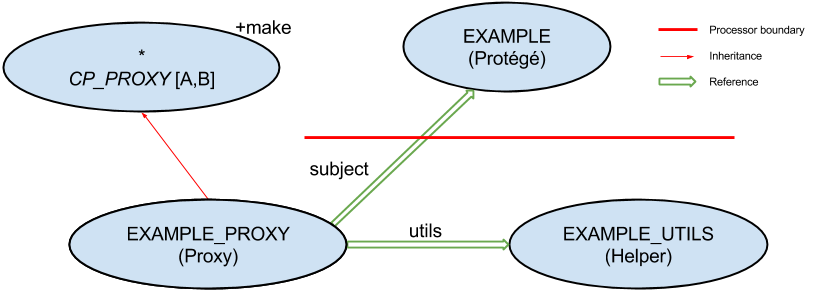
\includegraphics[width=\textwidth]{resources/separate_proxy.png}
\caption{The class relations in the Separate Proxy pattern.}
\end{figure}

Unfortunately this pattern cannot be turned into a reusable module, because it is highly dependent on the precise interface of the protégé class.
There is some support in the library however: 
\lstinline!CP_PROXY! defines a creation procedure and the attributes \lstinline!subject! for a separate protégé object and \lstinline!utils! for a helper object.

Appendix \ref{sec:howto-separate-proxy} provides a general recipe on how to implement a separate proxy for an arbitrary protégé class.

\subsection {Module overview}
\label{sec:module-overview}
% Describe available modules, which patterns they're implementing, and which modules they depend upon.
The library consists of several modules which implement some of the patterns described in the overview (Section \ref{sec:pattern_overview}).
The source code of the library is available on GitHub \cite{web:repository}.
All file locations in the following section are relative to the root directory of the repository.

One of the most basic modules is the import module in \dir{library/import}.
It implements the Import \patternref{IMP} pattern  and is at the same time one of the core concepts of the library.

The queue module in \dir{library/queue} implements the Prdocuer / Consumer \patternref{P/C} pattern.
It depends on the import module.

The process module in \dir{library/process} provides skeleton classes for objects with a main loop.
It provides implementations for the Active Object \patternref{AO}, Asynchronous Self-Call \patternref{ASC} and Timer: Periodic \patternref{TP} patterns.

The worker pool module in \dir{library/worker\_pool} implements the Worker Pool \patternref{WP} pattern.
It uses the import, queue and process module.

The directory \dir{library/promise} contains the promise module.
This module provides classes to monitor and interact with an asynchronous operation.

The executor module resides in \dir{library/executor} and provides an implementation to the Executor Framework \patternref{EF}, 
a specialized worker pool and part of the implementation to the Future pattern \patternref{FUT}.

The implementation of the future pattern is highly intertwined with other parts of the library.
It makes use of the promise, executor and worker pool modules and introduces only two classes on its own:
\lstinline!CP_COMPUTATION! and \lstinline!CP_FUTURE_EXECUTOR_PROXY!.

The class \lstinline!CP_DELAYED_TASK! in \dir{libary/util} implements the Timer: Invoke Later pattern \patternref{TIL}.
The same directory also contains the class \lstinline!CP_EVENT!, which implements the Publish / Subscribe pattern \patternref{P/S} in SCOOP.


\section{Library modules}
\label{sec:modules}

\subsection{Import}
\label{sec:modules:import}

The import module implements the SCOOP \lstinline!import! feature, which should be built-in but isn't implemented at the moment.
It is one of the most important modules of the library.
It consists of all classes in the directory \dir{library/import}.

The basic concepts on how to use the module is described in Section \ref{sec:concepts:import}.
This section only describes the descendants of \lstinline!CP_IMPORTER!, which provide predefined import functions for some types and support for writing an import feature manually.

The deferred class \lstinline!CP_IMPORTER [G]! defines the basic interface for a manually defined import feature.
To define an import feature for an arbitrary type, e.g. \lstinline!STRING!, one has to inherit from \lstinline!CP_IMPORTER [STRING]! and provide an implementation for the deferred \lstinline!import! feature.

Because writing an extra importer for every importable object may be tedious, there's a support class \lstinline!CP_IMPORTABLE!:

\begin{lstlisting}[captionpos=b, caption={The deferred class CP\_IMPORTABLE.}]
deferred class
  CP_IMPORTABLE

feature {CP_DYNAMIC_TYPE_IMPORTER} -- Initialization

  make_from_separate (other: separate like Current)
      -- Initialize `Current' with 
      -- the same values as `other'.
    deferred
    end

end
\end{lstlisting}

That way an import function can be written right inside the class that needs to be imported.

There are two classes which can be used for \lstinline!CP_IMPORTABLE! objects: \lstinline!CP_DYNAMIC_TYPE_IMPORTER! and \lstinline!CP_STATIC_TYPE_IMPORTER!.

The latter uses bounded genericity to directly create an object of type \lstinline!G!.
This has the drawback however that the type is statically \lstinline!G!, even if the argument to \lstinline!import! was of a subtype of \lstinline!G!.

The \lstinline!CP_DYNAMIC_TYPE_IMPORTER! tries to avoid this problem by using reflection.
This introduces a new problem with respect to void safety however, as the new object will not be initialized.
Therefore it is strongly advised to declare \lstinline!make_from_separate! as a creation procedure for every descendant of \lstinline!CP_IMPORTABLE!.

Another problem of the \lstinline!CP_DYNAMIC_TYPE_IMPORTER! are the invariants of an object.
There's a short time interval between the creation of an object (using reflection) and the call to \lstinline!{CP_IMPORTABLE}.make_from_separate! where the invariants are broken.
Due to this, it is not possible to have invariants in a class that will be imported using the dynamic type importer.

In the future, there will hopefully exist an import routine natively supported by the SCOOP runtime.
In that case \lstinline!CP_IMPORTER! can be made effective and use the native import, and all its descendants will become obsolete.


% Other components of the library often use the import module via bounded genericity.
% The class \lstinline!CP_QUEUE! for example has the ability to import objects, and it's class header looks like this:
% \begin{lstlisting}
% class CP_QUEUE
%   [G, IMPORTER -> CP_IMPORT_STRATEGY [G] create default_create end]
% feature
%   ...
% end
% \end{lstlisting}
% That way a user can decide on the precise semantics of the import strategy by just declaring the right type.

\subsection{Queue}

The queue module is a simple queue implementation in class \lstinline!CP_QUEUE!.
It is mostly used to easily implement the producer / consumer pattern in a concurrent context.


The pattern itself is all about data migration as described in Section \ref{sec:object-migration}.
Therefore the queue module makes heavy use of the import mechanism.
This means that, along with a generic argument for the data type, it is also necessary to provide a \lstinline!CP_IMPORT_STRATEGY!.
The import strategy then basically ``teaches'' the queue how to import a given object.

Internally, \lstinline!CP_QUEUE! uses an \lstinline!ARRAYED_LIST! to store its elements.

As the \lstinline!CP_QUEUE! is intended to be used as a separate object, the module provides support classes that implement the Separate Proxy pattern.

% It uses the separate proxy pattern, which means that it consists of three classes:
% 
% \begin{itemize}
%  \item \lstinline!CP_QUEUE!
%  \item \lstinline!CP_QUEUE_UTILS!
%  \item \lstinline!CP_QUEUE_PROXY!
% \end{itemize}
% 
% The first one provides the actual queue, but internally it just relies on \lstinline!ARRAYED_QUEUE!.
% The class \lstinline!CP_QUEUE_PROXY! can be used to access such a shared, separate queue without having to deal with separate references.
% 
% The interesting thing about this queue implementation is that it makes use of the import module.
% Along with the generic argument \lstinline!G! you can also provide an \lstinline!CP_IMPORT_STRATEGY [G]!.
% The import then happens automatically in both the queue and its proxy.

% \subsubsection{Producer / Consumer}
% 
% 
% The producer / consumer is a very popular pattern in concurrent programming, and it is a building block for other patterns like pipeline as well.
% The basic idea is to have a shared, concurrent buffer.
% Producer threads put new items into the buffer, whereas consumer threads remove items from this buffer.
% 
% \todo{BON-style diagram and ``migration graphics''}
% 
% In threaded systems, this buffer is usually accessed by several threads at the same time.
% Careful synchronization has to be enforced to ensure that the buffer remains in a consistent state.
% The data items on the other hand ``migrate'' from a producer to the buffer, and then to exactly one consumer.
% They therefore don't need to be thread-safe as long as the producer promises never to touch the item again.
% 
% In SCOOP things look a bit different however.
% Due to the exclusive access guarantee it is not necessary to establish a synchronization policy.
% The downside however is a loss of potential concurrency when a producer and a consumer accesses the buffer simultaneously, but this is a minor problem.
% 
% The main problem in SCOOP are the data items, especially if they are not of an expanded type.
% If the object is created on the producer processor, then the consumer needs to control the producer in order to get access to the object.
% This is clearly a situation that we want to avoid, because it couples the producer and consumer in a vicious hidden way, and the whole point of the producer / consumer pattern is to decouple the two.
% 
% A nice solution would be if it's somehow possible to migrate data items, like it's done in threaded languages.
% However, this is not possible with the current semantics of SCOOP, because an object always stays on the processor it was created on.
% 
% One approach to solve this problem is to create a new processor for every data item.
% This actually works, but it can be very slow, especially for a lot of small data items.
% There are two reasons for this:
% First, every SCOOP processor is mapped to an operating system thread, therefore creating a new processor involves creating a new thread which is an expensive operation.
% The second reason is the overhead of separate calls itself.
% This has to be paid every time the consumer wants to access the separate object.
% 
% Another problem of this approach is related to ease of programming.
% Dealing with a separate object can be very annoying, because you need to write small wrapper functions for every little feature call.
% 
% \begin{lstlisting}
% class
%   CONSUMER
% 
% feature -- Basic operations
%   
%   retrieve
%       -- Retrieve a string and print its length.
%     local
%       l_string: separate STRING
%     do
%       l_string := buffer_consume (a_queue)
%       print (string_count (l_string))
%     end
%     
% feature {NONE} -- Implementation
%   
%   buffer: separate BUFFER [STRING]
% 
%   buffer_consume (a_buffer: like buffer): separate STRING
%       -- An annoying small wrapper function for a buffer.
%     do
%       Result := a_buffer.item
%       a_buffer.remove
%     end
%     
%   string_count (a_string: separate STRING): INTEGER
%       -- An annoying small wrapper function for a string.
%     do
%       Result := a_string.count
%     end
% end
% \end{lstlisting}
% 
% 
% Due to these problems we decided to go for a different strategy: cloning objects.
% Using the import module it is possible to ``teach'' the shared buffer how to clone any user-defined object by just providing a generic argument.
% A first library for the producer / consumer pattern thus consisted of the class \lstinline!CP_QUEUE! and \lstinline!CP_IMPORT_STRATEGY!, along with some predefined importers.
% 
% The import trick solves the main problem of the producer / consumer, namely migrating objects from producer to consumer efficiently.
% However, producers and consumers still have to deal with a nasty separate reference (the shared buffer), and there's also the problem that a user of the library might forget to import objects on the consumer side.
% 
% To overcome this problem we implemented a non-separate proxy class which automatically deals with the separate reference and imports.
% This idea proved to be so successful that eventually it was turned into its own pattern: the separate proxy.
% 
% \todo {Bon-style graphics of CP\_QUEUE and related items.}


\subsection{Process}

The process module provides a set of classes that all implement some sort of skeleton for a main loop.

The class \lstinline!CP_PROCESS! defines the interface.
It is a descendant of the class \lstinline!CP_STARTABLE!, such that clients have a simple way to start a separate process using \lstinline!CP_STARTABLE_UTILS!.

The feature \lstinline!start! is used to start the main loop.
As the process module defines the skeleton for a main loop, users are just required to implement \lstinline!step!, which should contain the body of the loop.
The loop can be exited by setting the attribute \lstinline!is_stopped! to \lstinline!True!.

\lstinline!CP_PROCESS! also introduces the two methods \lstinline!setup! and \lstinline!cleanup!.
They are called in the beginning or at the end of the main loop, and must be explicitly redefined by descendants if needed.

There are two different implementations for the main loop itself.
The first, used by \lstinline!CP_CONTINUOUS_PROCESS!, is pretty staightforward:
\begin{lstlisting}
from setup
until is_stopped
loop
  step
end
\end{lstlisting}
The advantage of this approach is its simplicity.
However, other processors never get a chance to access data which is handled by the processor of the \lstinline!CP_CONTINUOUS_PROCESS!, unless the main loop is exited completely.
This class is a simple implementation of the \lstinline!Active Object! pattern \patternref{AO}.

The second implementation in \lstinline!CP_INTERMITTENT_PROCESS! is more interesting.
The basic idea is to perform only one iteration, and then tell another processor to inoke the loop body again in \lstinline!Current!.
This ping-pong approach ensures that after every iteration other processors may get a chance to access and modify data in \lstinline!CP_INTERMITTENT_PROCESS!.
In practice this is especially useful to stop a \lstinline!CP_INTERMITTENT_PROCESS! from the outside.

\lstinline!CP_INTERMITTENT_PROCESS! implements the Asynchronous Self-Call pattern \patternref{ASC}.
The callback service is provided by the class \lstinline!CP_PACEMAKER!, and every \lstinline!CP_INTERMITTENT_PROCESS! automatically creates an associated pacemaker.

The \lstinline!CP_PERIODIC_PROCESS! allows to add small delays between executions. 
It is a refinement of the \lstinline!CP_INTERMITTENT_PROCESS! and an implementation of the Timer: Periodic pattern \patternref{TP}.
The class also introduces the simple command \lstinline!stop!, which can be used to stop the process from the outside.


\subsection{Worker pool}
\label{sec:worker_pool} 

% The worker pool module provides support classes to build a worker pool.
% It makes use of the queue module to store the work items.
% 
% The module consists of three classes:
% 
% \begin{itemize}
%  \item \lstinline!CP_WORKER!
%  \item \lstinline!CP_WORKER_POOL!
%  \item \lstinline!CP_WORKER_FACTORY!
% \end{itemize}
% 
% The last one is just an factory class to create the user-defined \lstinline!CP_WORKER! objects.
% 
% The deferred class \lstinline!CP_WORKER! has a predefined main loop, where the object first checks if it needs to terminate, then grabs a new work item, and processes it.
% The processing step is deferred and needs to be implemented by the user.
% 
% The \lstinline!CP_WORKER_POOL! is the central management instance.
% Its primary task is to accept new work items from clients, but it can also be used to adjust the number of workers in the pool and to terminate all workers.
% The \lstinline!CP_WORKER_POOL! also implements the separate proxy pattern, which means that clients should access it through \lstinline!CP_WORKER_POOL_PROXY!.
% 
% \subsection{Worker pool}

A worker pool is a set of threads that are ready to execute tasks.
The intention of the worker pool is to make use of parallelism but avoid the overhead of thread creation, which can be quite expensive especially for small tasks.

The main component of the worker pool is a shared buffer, where clients can insert tasks to be executed.
A worker thread will then repeatedly retrieve a task from the buffer and execute it.
The worker pool module makes use of the queue module, which provides the shared buffer.
  %producer / consumer pattern, with the library client as a producer and the worker threads as consumers.

%An important part of the worker pool is also the ability to increase or decrease the amount of worker threads, or to completely stop all worker threads such that the application can terminate.

The representation of a task to be executed varies between different languages.
In Java for instance a Runnable object is used, whereas in C\# the task is represented as a delegate.

In SCOOP there's the problem of object migration, as described in Section \ref{sec:object-migration}.
If the task object is created on its own processor, as in the Data Processor approach, you cancel out the performance gain you tried to achieve with the worker pool.
With the Lock Passing approach, a task object will be executed on the processor that created the object, which kind of makes the worker pool useless (not to mention the risks of processor starvation if applied wrong).
This only leaves the Import mechanism as a sensible solution.

In the library we support two flavors of a worker pool.
The first and more basic one is to have a deferred class \lstinline!CP_WORKER! where clients can directly implement an operation.
The object submitted to the worker pool then corresponds to the arguments of the operation.

The second solution uses a special task class to encapsulate an operation.
It is described in Section \ref{sec:arbitrary-operations}.

% However, there are two solutions to this problem: You can either use the import mechanism, or make the worker class deferred and let clients implement the task directly.
% In the library we support both approaches, although the latter can be used to implement the import solution.
% Section~\ref{sec:arbitrary-operations} shows how to do this.

The basic worker pool module has three main classes:
\begin{itemize}
 \item \lstinline!CP_WORKER_POOL!
 \item \lstinline!CP_WORKER!
 \item \lstinline!CP_WORKER_FACTORY!
\end{itemize}

The \lstinline!CP_WORKER_POOL! provides the shared buffer and some additional functionality to adjust the pool size.
The type of the task object alongside its import strategy can be specified with a generic argument.
\lstinline!CP_WORKER_POOL! inherits from \lstinline!CP_QUEUE! and therefore uses the same import mechanisms.

The deferred class \lstinline!CP_WORKER! corresponds to the worker thread in other languages.
Users need to implement the feature \lstinline!do_run!, which takes a task object and executes it.
The exact type of the task object depends on the generic arguments of \lstinline!CP_WORKER!, which must be the same as in \lstinline!CP_WORKER_POOL!.
The non-deferred part in \lstinline!CP_WORKER! is the main loop itself, which fetches a new task, calls \lstinline!do_run!, and checks if the worker needs to terminate.

The last class, \lstinline!CP_WORKER_FACTORY!, just provides a deferred factory function for a new worker.
The factory class is necessary because the exact type of \lstinline!CP_WORKER! is not known to the library.
With a user-defined factory, the \lstinline!CP_WORKER_POOL! can create new workers on demand.




% \subsubsection{Terminating workers}

An important functionality of a worker pool is to adjust the number of workers.
Increasing the worker count is not a problem, as you can just create new \lstinline!CP_WORKER! instances using the factory.
To decrease the amount of workers, the module makes use of the processor termination technique described in Section \ref{sec:processor-termination}.


% However, decreasing the amount of workers is not that easy.
% 
% Java provides two builtin mechanisms to shut down a thread.
% You can either force it to stop, which immediately throws an exception in the thread \todo{ref}, or you can use the more collaborative interrupt mechanism \todo{ref}.
% The idea is that the thread will regularly check its interrupted flag and terminate on its own if requested.
% 
% The latter is also possible to do in SCOOP, except that there's no builtin interrupt flag.
% Instead a query \lstinline!is_stop_requested! in \lstinline!CP_WORKER_POOL! can be used.
% The main problem however are wait conditions.
% 
% In Java, blocking calls like \lstinline!wait()! and \lstinline!sleep()! may throw an \lstinline!InterruptedException! \todo{ref}.
% This avoids the problem that a thread may wait forever instead of shutting down, because all signaller threads have already terminated.
% Unfortunately, there's no such mechanism in SCOOP.
% It is possible however to work around this limitation by refining the wait condition:
% \begin{lstlisting}
% 
% class
%   CP_WORKER
%   
%   -- ...
%   
% feature -- Implementation
% 
%   fetch (pool: separate CP_WORKER_POOL)
%     require
%       not pool.is_empty or pool.is_stop_requested
%     do
%       if is_stop_requested then
% 	-- Stop the currrent worker.
%       else
% 	-- Grab the next item.
%       end
%     end
% 
% end
% \end{lstlisting}
% The additional \lstinline!if! statement is not very nice, but luckily it can be encapsulated completely in \lstinline!CP_WORKER!.
% 
% This code snippet is useful to break free of any wait condition if the requirements have changed.


The Separate Proxy pattern is applied to \lstinline!CP_WORKER_POOL! to simplify the use of a separate worker pool object.

The basic worker pool module allows for a very flexible use. 
It is for example possible to use it just as an advanced producer / consumer module where consumers are automatically created and destroyed.
The next section introduces a more advanced implementation of the worker pool which builds on the basic module.



\subsubsection{Arbitrary operations}
\label{sec:arbitrary-operations}

So far the task of a worker is defined in a user-defined \lstinline!CP_WORKER! class, and the object submitted to the worker pool mostly contains data.
The worker pool implementations in Java and C\# only accept Runnable (or delegate) objects.
This enables arbitrary operations that can be executed by the worker threads.

The SCOOP version of the worker pool can be enhanced to act like the Java / C\# counterparts.
To do that we need a class that represents an operation, and which can be moved across processor boundaries.

The agent classes in Eiffel (i.e. ROUTINE and descendants) may be used to represent operations, but they can't be easily imported.
That's why we added a new, deferred class \lstinline!CP_TASK!.
Users of the library can inherit from it and implement the feature \lstinline!run!.
\todo {Tell about agent integration?}

Using this interface it is possible to have a predefined \lstinline!CP_TASK_WORKER! that just runs \lstinline!CP_TASK! objects.
The associated \lstinline!CP_TASK_WORKER_POOL! implements the factory function and refines the raw \lstinline!CP_WORKER_POOL!.

The combination of these two classes is very close to the Java worker pool implementation.
The only difference is that a \lstinline!CP_TASK! object needs to be imported, whereas a Java Runnable object doesn't.


\todo{Maybe merge subsections Arbitrary Operations and Promise into a new section that describes the ideas behind CP\_TASK?}

\subsection{Futures}
\label{sec:futures}

The future pattern is used to perform a computation asynchronously.
Instead of computing a value directly, the computation gets wrapped into an object and the user only receives a handle to retrieve the value when it's ready.
This handle is often called Future, Promise or Delay.
In this section we'll use the term Future for the whole pattern, and Promise only refers to the handle.

The main advantage of the future pattern is that it allows to make use of parallelism in an easy way.
A user just has to spot computations which may run asynchronously, and the future pattern takes care of thread management, synchronization and result propagation.

The future pattern consists of four building blocks:
\begin{itemize}
 \item The Promise object,
 \item the computation,
 \item the execution service,
 \item and a ``frontent'' object which takes a computation, submits it to the executor, and returns a Promise object.
\end{itemize}

The representation of the computation is a Callable object in Java and a delegate in C\#.
Our library uses the interface \lstinline!CP_COMPUTATION! with the deferred feature \lstinline!computed!.
It is a descendant of \lstinline!CP_TASK! introduced in Section \ref{sec:arbitrary-operations}.

The Promise object is defined by \lstinline!CP_PROMISE! and its descendants.
The detailed implementation is described in Section \ref{sec:promise}.

The execution service part of the Future pattern can vary.
In most cases it is a worker pool which executes the computation objects and updates the Promise with the correct result.
However, it is also possible to implement it as a single thread, or even to executing them synchronously in the current thread.

To take this variation into account, we added the interface \lstinline!CP_EXECUTOR!.
The \lstinline!CP_TASK_WORKER_POOL! introduced in Section \ref{sec:worker_pool} implements this interface and thus can be used as an executor service for the Future pattern.
We also applied the Separate Proxy pattern on \lstinline!CP_EXECUTOR!, as it is mostly accessed through a separate reference.

\todo {Maybe highlight that EXECUTOR is not just for the future pattern, but a general implementation of the Executor pattern.}

The ``frontend'' part is implemented in the \lstinline!CP_EXECUTOR_PROXY!.
This is an example where the responsability of a proxy object has been expanded:
Instead of just forwarding the \lstinline!CP_COMPUTATION! to the execution service, it also creates the Promise object and returns it to the user.

The implementation of the future pattern in SCOOP hits two challenges:
\begin{itemize}
 \item Object Migration (see Section \ref{sec:object-migration}: Operations can't be easily moved from the client to an execution service.
 The same is also true for the result of a computation in the reverse direction.
 \item Processor Communication (see Section \ref{sec:processor-communication}: The promise object should neither be placed on the client processor nor on the executor service.
% The reason in both cases is that one processor may execute a main loop, which means the other processor never gets access to the promise object.
\end{itemize}

The solution to the first problem is, once again, the import concept (Section \ref{sec:concepts:import}.
% This means that both the Executor service and the Promise object have a generic argument to define the \lstinline!CP_IMPORT_STRATEGY!.
% The executor service always uses \lstinline!CP_DYNAMIC_TYPE_IMPORTER!, because \lstinline!CP_COMPUTATION! inherits from \lstinline!CP_IMPORTABLE!.
% The import strategy of the Promise object however is user-defined.
The second problem is more interesting however.
As we've seen in Section \ref{sec:processor-communication}, the Promise object needs to be placed on a third processor.

However, if we start a new processor for every computation, we introduce a huge overhead.

A better tradeoff would be to introduce one global processor, which takes care of all promise objects.
This may introduce contention if multiple futures are submitted, but we think that this is acceptable.

However, this approach brings another problem.
A promise object has two generic arguments for the return type and the import strategy.
As these arguments are not known in advance, and because SCOOP processor tags \cite[p. 90]{Nienaltowski07} are not implemented yet, it is not possible to create a promise object on this dedicated processor.

The solution is - surprisingly - the import module.
We can create a promise object with the correct types on the client processor, and then ask the global processor to import it.
This way the promise object finally ends up on the correct processor.

% In the library, the Promise object is provided by the class \lstinline!CP_PROMISE! and its descendants.
% The computation is represented with \lstinline!CP_COMPUTATION!, or \lstinline!CP_TASK! for operations that don't return a result.
% The execution service is the deferred class \lstinline!CP_EXECUTOR! and \lstinline!CP_TASK_WORKER_POOL! is the main implementation.
% 
% The separate proxy pattern is applied on \lstinline!CP_EXECUTOR! and \lstinline!CP_PROMISE!.
% Besides acting as a processor-local proxy to a separate \lstinline!CP_EXECUTOR!, 
% the classes \lstinline!CP_EXECUTOR_PROXY! and \lstinline!CP_FUTURE_EXECUTOR_PROXY! are also responsible to create Promise objects on the global processor.

\subsubsection{Promise}
\label {sec:promise}

The promise module contains a set of classes which can be used to monitor the state of an asynchronous operation.

The main class is \lstinline!CP_PROMISE!, which defines queries like \lstinline!is_terminated! or \lstinline!is_exceptional!.
It also defines the interface to cancel a task or to get the progress percentage (e.g. for a download task), but these queries need to be supported by the task itself.

The Separate Proxy mechanism is available for promise objects, because they are usually declared separate to the client.
In this case the pattern is implemented with four classes, i.e.
\begin{itemize}
 \item \lstinline!CP_PROMISE! defines a common interface,
 \item \lstinline!CP_SHARED_PROMISE! defines the actual separate object,
 \item \lstinline!CP_PROMISE_UTILS! introduces helper functions to access a \lstinline!separate! \lstinline!CP_PROMISE! and
 \item \lstinline!CP_PROMISE_PROXY! is the proxy object.
\end{itemize}

There's an important descendant, the \lstinline!CP_RESULT_PROMISE!, which is used for asynchronous operations that return a result.
It also has a set of associated classes that implement the Separate Proxy pattern.

The \lstinline!CP_RESULT_PROMISE! contains a query \lstinline!item! to retrieve the result as soon as it's available.
A distinguishing feature of this query is that it blocks if the result is not yet available.
The return type of \lstinline!item! depends on a generic argument.
To migrate the result back to the client, this class makes use of the import module - i.e. the \lstinline!CP_SHARED_RESULT_PROMISE! and \lstinline!CP_RESULT_PROMISE_PROXY! both have an additional generic argument which defines the import strategy.

% The \lstinline!CP_RESULT_PROMISE! is used for the future pattern.

% \subsubsection{Executor}
% 
% The executor module can be used to execute varying operations.
% The main class is \lstinline!CP_EXECUTOR!, which provides facilities to execute a \lstinline!CP_TASK! objects.
% 
% \lstinline!CP_TASK! itself represents a user-defined operation.
% It can be imported across processor boundaries and provides exception handling.
% To define a new task a client needs to inherit from \lstinline!CP_DEFAULT_TASK! and implement the feature \lstinline!run! and \lstinline!make_from_separate!.
% 
% A special kind of task is \lstinline!CP_COMPUTATION!, which can also return a value.
% This is needed to implement the future pattern.
% 
% The \lstinline!CP_EXECUTOR! makes use of the separate proxy pattern.
% However, the proxy also enhances the raw \lstinline!CP_EXECUTOR! interface with the option to attach a \lstinline!CP_PROMISE! object to a task.
% This can be used to query the status of a task, await termination, or get the computed result back in case of a \lstinline!CP_COMPUTATION!
% All \lstinline!CP_PROMISE! objects are created on a dedicated processor to avoid unnecessary thread creation.
% 
% An important implementation of the \lstinline!CP_EXECUTOR! is the \lstinline!CP_TASK_WORKER_POOL!.
% As the name suggests, this is a worker pool where each worker repeatedly executes \lstinline!CP_TASK! objects.
% 
% \todo {More executor implementations?}


\section{Evaluation}
\label {sec:evaluation}

To evaluate the library we did a small performance benchmark.
We implemented the Gaussian elimination algorithm in three different ways: sequentially, with SCOOP only, and using the future module (see Section \ref{sec:futures}) from our library.
We chose to use the future module because it indirectly also measures many other parts of the library like the worker pool or import mechanism.

We ran the tests with randomly generated square matrices.
The order of a matrix was always a power of two in the range from 32 to 1024.
Additionally, there was one more column for the result vector in the system of linear equations.
Each test was repeated 5 times.
The test system was a quad-core AMD Phenom II X4 955 processor with 6 GB of RAM.
The results are shown Table \ref{table:perf-results}.

\begin{table} [h]
\centering
\begin{tabular}{|l|l l l|} 
\hline
Matrix Size & Future & Raw SCOOP & Sequential\\
\hline
32 & 0.36 & 0.19 &  \textless 0.01\\
64 & 1.67 & 1.11 & \textless 0.01\\
128 & 8.45 & 9.27 & 0.04\\
256 & 26.45 & 66.56 & 0.33\\
512 & 102.28 & 515.11 & 2.62\\
1000 & - &  3937.2 & - \\
1024 & 424.32 & error & 20.79 \\
\hline
\end{tabular}
\caption{Average time in seconds for different algorithms.}
\label{table:perf-results}
\end{table}

We can get several observations from the results:

\begin{itemize}
 \item The raw SCOOP solution fails for the biggest matrix.
 This is a known bug \cite{web:scoop-issues}:
 The algorithm uses more than the maximum number of processors.
 The library solution doesn't suffer from this problem because it's using a fixed amount of processors.
 \item Futures are faster than raw SCOOP for large data sets.
 \item For smaller data sets, raw SCOOP beats the library.
 \item Sequential execution is much faster than SCOOP.
\end{itemize}

The last observation is probably the most fundamental.
The SCOOP runtime really needs to be improved in order to make it competitive to threaded systems, or even sequential ones.
Fortunately an improved version \cite{thesis:scottwest} is being developed at the time of writing.
It will probably be integrated into a future EiffelStudio release.

Another improvement which might be useful for the library is the Passive Processor concept \cite{paper:passive-processors}.
If both the worker pool and the promise processor could be declared passive the computation speed up a lot.

\section{Conclusion}
% Explain what is the impact of the selected patterns, and why they were selected.
% Say that import was developed to overcome language limitation
% Also: Future work

Concurrent programming is increasingly becoming the norm despite its difficulties.
The SCOOP model provides a solid foundation to concurrent programming in Eiffel, 
but it is hard to learn for developers due to the paradigm shift and the lack of a concurrency library.

In this thesis we've worked out many methods that simplify concurrent programming in SCOOP.
We did a broad survey of popular concurrency patterns and present our findings in a detailed list.
The list can be used to search for a pattern that fits a particular problem, which may even be useful to programmers of threaded languages.

From our survey we selected some patterns which we thought to be especially useful.
The selection was based on the study of other concurrency libraries as well as some input from the Software Engineering research group at ETH.
The seleted patterns were then implemented and are now available as a new Eiffel library.
Besides the pattern implementations, the library also provides some workarounds for current SCOOP limitations, such as the missing import statement.

Performance measurements for the Future pattern showed that the library is actually faster for large data sets and uses less threads than the native SCOOP approach.

Finally, we also described some challenges when programming in SCOOP and how to solve them.
This is especially useful to developers experienced in threaded programming who want to use SCOOP for the first time.

\subsection{Future work}

The library provides several opportunities for future work.

\begin{description}
 \item [More patterns] The library can be extended with additional patterns.
 It may be useful to include Pipeline or Dataflow Network.
 \item [Separate Proxies] The Separate Proxy pattern may be applied to some EiffelBase classes, such as \lstinline!ARRAYED_LIST!, \lstinline!HASH_TABLE! or \lstinline!ROUTINE!.
 \item [Separate Proxy Wizard] Writing a Separate Proxy is tedious. Most of it could be automated with a wizard however.
 \item [Concurrent Datastructures] Sometimes it may be useful to have truly concurrent data structures for performance reasons.
The Array Slicing technique \cite{paper:array-slicing} is an example how arrays with concurrent read access can be implemented in SCOOP.
\end{description}

SCOOP itself also provides a rich offering of possible improvements.

\begin{description}
 \item [Faster runtime] The SCOOP runtime needs to become faster. 
 This is currently being developed \cite{thesis:scottwest}.
 \item [Native Import] A native SCOOP import mechanism is a great tool to deal with a lot of small objects.
 It will also make the library API and implementation simpler, as the manual import workaround can be removed.
 \item [Passive Processors] The passive processors concept \cite{paper:passive-processors} could be integrated into EiffelStudio.
 It can make a big performance improvement to situations where one needs to pass data from one processor to another.
 \item [Separate references] The handling of separate references should become more convenient.
 At the moment programmers are forced to write a lot of small, annoying features to perform separate calls.
 Some syntactic sugar would be really helpful.
\end{description}

\newpage
\begin{appendices}
\section{How-To: Separate Proxy}
\label{sec:howto-separate-proxy}

This appendix shows how to implement a separate proxy based on a small class \lstinline!EXAMPLE!.

\begin{lstlisting} [captionpos=b, caption={The example class (protégé) where the separate proxy should be applied.}]
class interface
  EXAMPLE [G]

feature -- Status report

  is_available: BOOLEAN
      -- Is `item' available?
  
feature -- Access

  item: separate G
      -- Item in `Current'.
    require
      available: is_available

feature -- Element change

  put (a_item: separate G)
      -- Set `item' to `a_item'.

end
\end{lstlisting}

First we need to create the helper class.
This is done according to these rules:
 \begin{itemize}
  \item The name should end in \lstinline!_UTILS!, i.e. \lstinline!EXAMPLE_UTILS!.
  \item The generic arguments are the same as in \lstinline!EXAMPLE!.
  \item Any feature to access the separate \lstinline!EXAMPLE! object should be prefixed with \lstinline!example_!.
  This helps to avoid name clashes if someone wants to inherit from \lstinline!EXAMPLE_UTILS!.
  \item The first argument of each feature is \lstinline!example: separate EXAMPLE [G]!.
  All other arguments are the same as the ones in the corresponding feature in \lstinline!EXAMPLE!.
  \item Preconditions in \lstinline!EXAMPLE! should be rewritten as wait conditions with the same meaning in \lstinline!EXAMPLE_UTILS!.
  \item If there's a non-expanded return type to a feature, you can decide if it should be declared separate in \lstinline!EXAMPLE_UTILS! or if it should be imported.
 \end{itemize}

\begin{lstlisting} [captionpos=b, caption={The helper class for a separate EXAMPLE.}]
class
  EXAMPLE_UTILS [G]
  
feature -- Access

  example_item (example: separate EXAMPLE [G]): separate G
      -- Get the item from `example'.
      -- May block if not yet available.
    require
      available: example.is_available
    do
      Result := example.item
    end

feature -- Element change
 
  example_put (example: separate EXAMPLE [G];
	    item: separate G)
      -- Put `item' into `example'.
    do
      example.put (item)
    end
end
\end{lstlisting}

In this example we also dropped the feature \lstinline!is_available!, because it's not considered to be important for separate clients.

The proxy class also has some simple rules:

 \begin{itemize}
  \item The name should be \lstinline!EXAMPLE_PROXY!.
  \item The generic arguments are the same as in \lstinline!EXAMPLE!.
  \item Inheriting from \lstinline!CP_PROXY [EXAMPLE [G], EXAMPLE_UTILS [G]]! is recommended.
  That way one can avoid having to write the creation procedure \lstinline!make!.
  \item The feature names and arguments are the same as in \lstinline!EXAMPLE!.
  \item Preconditions in \lstinline!EXAMPLE! are not present in \lstinline!EXAMPLE_PROXY!. 
  The class \lstinline!EXAMPLE_UTILS! defines them as wait conditions instead.
  \item Every feature body makes use of \lstinline!utils! to forward its requests to the \lstinline!subject!.
 \end{itemize}

\begin{lstlisting} [captionpos=b, caption={The proxy class for a separate EXAMPLE.}]
class
  EXAMPLE_PROXY [G]

inherit
  CP_PROXY [EXAMPLE [G], EXAMPLE_UTILS [G]]

create
  make
  
feature -- Access

  item: separate G
      -- Item in the example object.
      -- May block if not yet available.
    do
      Result := utils.example_item (subject)
    end

feature -- Element change

  put (a_item: separate G)
      -- Set `item' to `a_item'.
    do
      utils.example_put (subject, a_item)
    end

end
\end{lstlisting}

\section{SCOOP and EiffelVision}

At the core of most GUI toolkits is an event dispatching thread (EDT).
The EDT is running an infinite loop where it listens for user input events.

Only the EDT is allowed to modify user interface objects.
Background threads therefore have to enqueue agents to be executed by the EDT if they want to update the GUI.

EiffelVision also follows this design with the event dispatching code defined in \lstinline!EV_APPLICATION! and the enqueuing feature \lstinline!do_once_on_idle! in the same class.
Due to this design one might think that combining SCOOP with EiffelVision is impossible.

This is not true however.
EiffelVision implements a variation of the Asynchronous Self-Call pattern \patternref{ASC}.
The body of the loop is defined by the feature \lstinline!{EV_APPLICATION_I}.process_event_queue!, whereas the actual loop is implemented in \lstinline!EV_APPLICATION_HANDLER!.
Therefore, a user interface object can subscribe to events from separate processors in the same manner as it can subscribe to events from the same processor.

In fact the SCOOP model makes GUI programming a lot easier.
In threaded languages programmers constantly have to worry that only the EDT manipulates user interface objects.
SCOOP however gives this guarantee for free.
This completely eliminates a source of randomly occurring errors which are usually very hard to find.

We'll show a small example application which can download a file in the background.
The application has a simple graphical user interface and uses the executor module from the library.
Some highlights of the example are event propagation and the cancellation mechanism.
The full source code can be found in \dir{examples/eiffelvision\_downloader} in the repository \cite{web:repository}.

Let's first look at the business logic.
The class \lstinline!DOWNLOAD_TASK! in Listing \ref{code:download-task} defines the background downloader.
It inherits from \lstinline!CP_DEFAULT_TASK! such that it can be used in conjunction with an executor.

\begin{lstlisting}[language=OOSC2Eiffel, label={code:download-task}, captionpos=b, caption={The background download task.}]
class
	DOWNLOAD_TASK

inherit
	CP_DEFAULT_TASK

    -- Initialization omitted.

feature -- Access

	url: STRING

feature -- Basic operations

	run
			-- <Precursor>
		local
			download_fragments: ARRAYED_LIST [STRING]
			http_downloader: detachable HTTP_PROTOCOL
			size: INTEGER
		do
			create download_fragments.make (50)
			create http_downloader.make (create {HTTP_URL}.make(url))

			from
					-- Start the download
				http_downloader.set_read_mode
				http_downloader.open
				http_downloader.initiate_transfer
				size := http_downloader.count
			until
					-- Terminate when the download is finished 
					-- or the user cancels the download manually.
				http_downloader.bytes_transferred = size 
				or attached promise as l_promise 
				and then is_promise_cancelled (l_promise)
			loop
					-- Receive a single packet.
				http_downloader.read
				if attached http_downloader.last_packet as l_packet then
					download_fragments.extend (l_packet)
				end
					-- Update the progress information in the UI.
				if attached promise as l_promise then
					promise_set_progress (l_promise, 
					  http_downloader.bytes_transferred / size)
				end
			end

				-- Discard result. A real application would
				-- probably write it to a file
			download_fragments.wipe_out
			http_downloader.close
		rescue
			if attached http_downloader as dl and then dl.is_open then
				dl.close
			end
		end
end
\end{lstlisting}

The code is structured such that the loop body only handles a small chunk of the total download.
This allows to check for a cancellation request in regular intervals, and to publish the current progress to the shared promise object.

The rescue clause at the end ensures that the connection is correctly closed.
Note that this is the only exception handling which needs to be done, and it's not necessary to ``catch'' an exception with \lstinline!retry!.
The user interface is still safe though because the exception gets caught later, transformed to an unsuccessful termination event, and the GUI will be informed automatically.

Another major component is the class which defines the main window.
It contains a lot of boring EiffelVision initialization code however.
Listing \ref{code:main-window} therefore only shows the event handling part.

\begin{lstlisting}[language=OOSC2Eiffel, label={code:main-window}, captionpos=b, caption={The main window.}]
class
	MAIN_WINDOW
inherit
	EV_TITLED_WINDOW

			-- Initialization and GUI elements omitted.

feature -- Access

	executor: CP_EXECUTOR_PROXY
			-- An executor to submit background tasks to.

	download_handle: detachable CP_PROMISE_PROXY
			-- A handle to a possible background download.

	formatter: FORMAT_DOUBLE
			-- A formatter for progress values.

feature -- Status report

	is_cancelling: BOOLEAN
			-- Is the download about to terminate?
			
feature {NONE} -- Button press events

	on_download_button_clicked
			-- Handler for clicks on download button.
		local
			downloader: DOWNLOAD_TASK
			l_promise: CP_PROMISE_PROXY
		do
			if not attached download_handle then

				create downloader.make (url_text.text)
				l_promise := executor.new_promise
				download_handle := l_promise

				l_promise.progress_change_event.subscribe (agent on_progress)
				l_promise.termination_event.subscribe (agent on_terminated)

				downloader.set_promise (l_promise.subject)
				executor.put (downloader)
			end
		end

	on_cancel_button_clicked
			-- Handler for clicks on cancel button.
		do
			if 
			   not is_cancelling and 
			   attached download_handle as l_download
			then
				l_download.cancel
				is_cancelling := True
				status_text.set_text ("Cancelling download...")
			end
		end

feature {NONE} -- Background download events

	on_terminated (is_successful: BOOLEAN)
			-- Handler for termination events from download task.
		do
			if not is_successful then
				result_text.set_text ("Download aborted.")
			elseif is_cancelling then
				result_text.set_text ("Download cancelled.")
				is_cancelling := False
			else
				result_text.set_text ("Download finished.")
			end

			status_text.set_text ("No download in progress.")
			download_handle := Void
		end

	on_progress (progress: DOUBLE)
			-- Handler for progress change events from download task.
		do
			if not is_cancelling then
				status_text.set_text ("Download progress:" +
				    formatter.formatted (progress * 100) + "%%")
			end
		end
end
\end{lstlisting}

The most interesting feature is \lstinline!on_download_button_clicked!.
It starts a background task and sets up all event handlers such that the user interface can react to progress change or termination events.
The events are predefined in \lstinline!CP_PROMISE! and sent automatically to all subscribers whenever the associated task changes the progress value or terminates.

The \lstinline!on_terminated! handler function is used to receive an event that the background task has finished.
There are three cases that need to be distinguished: normal termination without cancellation, normal termination with cancellation, and exceptional termination due to an error.

The last component is the class \lstinline!DOWNLOAD_APPLICATION!.

\begin{lstlisting}[language=OOSC2Eiffel, label={code:download-application}, captionpos=b, caption={Download application root class.}]
class
	DOWNLOAD_APPLICATION

create make

feature {NONE} -- Initialization

	make
			-- Start the download application example.
		local
			app: EV_APPLICATION
			main_window: MAIN_WINDOW
			worker_pool: separate CP_TASK_WORKER_POOL
		do
				-- Create a worker pool which can be 
				-- used to execute background downloads.
			create worker_pool.make (10, 1)
			create executor.make (worker_pool)

				-- Create application and main window.
			create app
			create main_window.make (executor)

				-- Don't forget to tear down the worker pool at the end.
			app.destroy_actions.extend (agent executor.stop)

				-- Start the GUI.
			main_window.show
			app.launch
		end

feature -- Access

	executor: CP_EXECUTOR_PROXY
			-- The worker pool for background tasks.

end
\end{lstlisting}

The class just creates and launches the event loop, the worker pool and the main window.
The most interesting part is how the worker pool can be stopped.
As the statement \lstinline!app.launch! just kick-starts the event loop and then returns we can't destroy the worker pool after this statement as in a sequential program.
It is therefore necessary to install a handler to stop the executor when the event loop terminates.



\section {API tutorial}
\label{sec:tutorial}

\subsubsection{Producer / Consumer}

The producer / consumer example is pretty common in concurrent programming.
At its core is usually a shared buffer.
A producer can add items to the buffer, whereas a consumer removes items from the buffer.

The library class \lstinline!CP_QUEUE! can be used as a shared buffer.
If we want to use \lstinline!STRING! objects to be passed from producer to consumer, we have to declare the queue like this:

\begin{lstlisting}
class PRODUCER_CONSUMER feature

  make
      -- Launch producers and consumers.
    local
      queue: separate CP_QUEUE [STRING, CP_STRING_IMPORTER]
	-- ...
    do
      create queue.make_bounded (10)
	-- ...
    end
end
\end{lstlisting}

Note that there are two generic arguments:
\begin{itemize}
\item The first argument (\lstinline!STRING!) denotes the type of items in the queue.
\item The second argument (\lstinline!CP_STRING_IMPORTER!) defines the import strategy.
\end{itemize}

The import strategy is an important concept of the library.
An import in the SCOOP context means that an object on a separate processor should be copied to the local processor.
This is done recursively for any non-separate reference, i.e. for  \lstinline!STRING! you also have to copy the \lstinline!area! attribute.
The import strategy can be used to tell a component if a given object should be imported, and if yes, how it is done.

In our example we're using the \lstinline!CP_STRING_IMPORTER! to import strings.
An alternative would be to use \lstinline!CP_NO_IMPORTER [STRING]! if we want to disable imports.

The next step we need to do is to define the producer and consumer.

\lstinputlisting [firstline=7] {../../examples/producer_consumer/producer.e}

You may notice three things in this example:

\begin{itemize}
 \item \lstinline!PRODUCER! inherits from \lstinline!CP_STARTABLE!.
 \item The \lstinline!PRODUCER! uses a \lstinline!CP_QUEUE_PROXY! instead of the \lstinline!CP_QUEUE!.
 \item The generated strings are not separate.
\end{itemize}

The classes \lstinline!CP_STARTABLE! and \lstinline!CP_STARTABLE_UTILS! are a useful combination.
They allow to start some operation on a separate object without the need for a specialized wrapper function.

Another nice utility is the \lstinline!CP_QUEUE_PROXY!.
It is part of a pattern which is often used throughout the library - the separate proxy \todo{add reference}.
Basically it allows to access a separate queue without the need to deal with separate references.

The really interesting thing however is that the producer can generate strings on its local processor.
Usually this is not possible, because if the string is later passed to a consumer object, the latter needs to lock the producer in order to get access to the string.
But in this case we instructed the queue object to import all string objects. During a call to \lstinline!queue_wrapper.put(item)! the following happens:
\begin{itemize}
 \item The producer waits until it gets exclusive access to the queue.
 \item The separate call is executed. Because \lstinline!item! is a non-separate reference, the call is synchronous and lock passing happens.
 \item The queue object imports the separate string, creating a local copy.
 \item The separate call terminates, both processors can proceed autonomously.
\end{itemize}
Creating the strings on a separate processor is therefore unnecessary.

The import trick avoids a lot of unnecessary thread creation:
Instead of creating a new processor for every single produced item we just copy it, which is much faster for small objects.

The consumer is basically the same as the producer, except for the feature \lstinline!start!:

\begin{lstlisting}
class
  CONSUMER
--...
  
	start
			-- Consume `item_count' items.
		local
			i: INTEGER
			item: STRING
		do
			from
				i := 1
			until
				i > item_count
			loop
				queue_wrapper.consume

				check attached queue_wrapper.last_consumed_item as l_item then

						-- Note that `item' is not declared as separate, because it has been
						-- imported automatically.
					item := l_item
					print (item + " // Consumer " + identifier.out + ": item " + i.out + "%N")
				end
				i := i + 1
			end
		end
end
\end{lstlisting}

You might notice again that the consumed string is not declared as separate.
This is again because of the import mechanism within \lstinline!CP_QUEUE!.

The last thing we need to do is to create and launch the producers and consumers in the main application:

\lstinputlisting [firstline=7] {../../examples/producer_consumer/producer_consumer.e}


\subsubsection{Server thread}

In networking you often need a dedicated thread that listens on a socket.
In a SCOOP environment it is not hard to create such a processor, but it is hard to stop it.
The main problem is that the server processor will run its own main loop, and other threads ususally never get exclusive access to call some feature \lstinline!stop!.

The library addresses this issue with the \lstinline!CP_INTERMITTENT_PROCESS!.
This class defines a special main loop, where other processors can access the object after every iteration.

To use \lstinline!CP_INTERMITTENT_PROCESS! you need to inherit from it and implement the deferred feature \lstinline!step!.
The following example defines a simple echo server that just listens and replies with the same string:

\lstinputlisting [firstline=7] {../../examples/echo_server/echo_server.e}

To break out of the main loop, you need to set \lstinline!is_stopped! to \lstinline!True!.
This can be done from within the \lstinline!CP_INTERMITTENT_PROCESS! or from a separate processor by calling \lstinline!stop!.

To start the echo server you can use \lstinline!CP_STARTABLE_UTILS! and the feature \lstinline!asynch_start!:

\lstinputlisting [firstline=7] {../../examples/echo_server/echo_application.e}

\subsubsection{Futures}

A future is a computation which may run asynchronously, possibly returning a result.
The future is a very popular pattern in other languages like Java.

The idea is that the computation is encapsulated in an object which may be executed by another thread.
If there's a result to the computation, the client thread also gets a token back to access the result at some point in the future.
This token is usually called ``Future'' or ``Promise''.

The library mechanism to support futures are the class hierarchies rooted at \lstinline!CP_TASK!, \lstinline!CP_BROKER! and \lstinline!CP_EXECUTOR!.

The \lstinline!CP_DEFAULT_TASK! class is used to define the operation.
To use it you need to inherit from it and implement \lstinline!run! and \lstinline!make_from_separate!.
The latter is needed because SCOOP doesn't allow shared access to objects, which is why a \lstinline!CP_TASK! needs to be imported from one processor to another.
If the operation is returning a result, it is necessary to inherit from \lstinline!CP_COMPUTATION! and implement \lstinline!computed!.

\lstinline!CP_EXECUTOR! is used to submit a task to be executed.
The main implementation is \lstinline!CP_TASK_WORKER_POOL!, which is using a worker pool to execute \lstinline!CP_TASK! objects.
The executor shoud be accessed using a local \lstinline!CP_EXECUTOR_PROXY! and \lstinline!CP_FUTURE_EXECUTOR_PROXY!, which simplify access to the \lstinline!separate CP_EXECUTOR! and also initialize the Promise object.

The \lstinline!CP_BROKER! serves as the token to store the status of the computation and a possible result.
It is created on a separate processor, such that both the client and the task object can access it without the risk of a deadlock.
If you use \lstinline!CP_EXECUTOR_PROXY!, you can submit a task and receive a token object by using \lstinline!put_with_broker!.

\todo{integrate example} 

\end{appendices}

\newpage
\phantomsection
\addcontentsline{toc}{section}{References}
\begin{flushleft}
{{{
\bibliographystyle {plain}
\bibliography {./resources/references}
}}}
\end{flushleft}

\end{document}          
